\begin{figure}[t]
\begin{center}
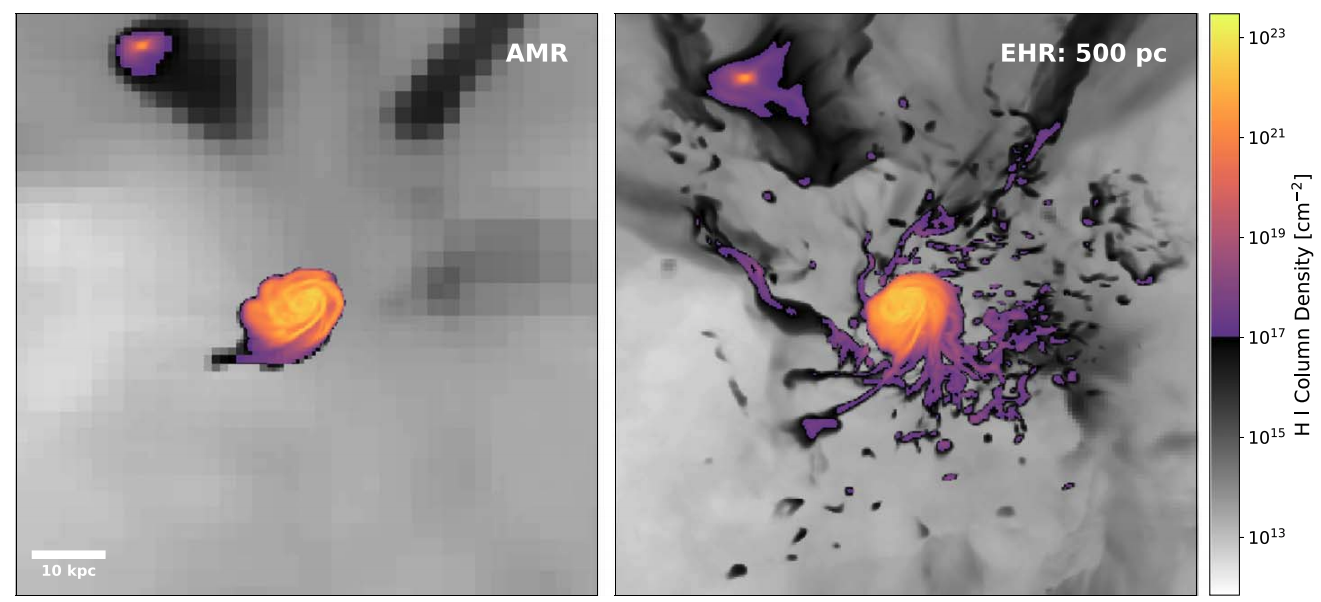
\includegraphics[width=0.99\textwidth]{EHR.png}
\end{center}
\vspace{-6mm}
\caption{\label{fig:ehr} 
Two simulations using the \emph{Tempest} suite of simulations
\citep{Hummels19}. The figure on the right has had enhanced halo resolution
(EHR) which causes striking differences in the morphology of the gas around the galaxy.
This will impact the evolution and structures of the magnetic field in the
galaxy by altering the ability of the galaxy to expel flux.
%Coherent magnetic structure is seen in
%many disk galaxies. (\emph{Left}) The magnetic field from
%polarized $\lambda=3,6$ and 20 cm  radio emission (vectors) along with total
%emission (contours) in M51. From  \cite{Fletcher11}.  Optical background from \emph{Hubble Space Telescope}
%(image credit: NASA, ESA, S. Beckwith (STScI) and The Hubble Heritage Team
%(STScI/AURA)).  This shows the well-ordered nature of the magnetic field along
%the spiral arms. 
%(\emph{Right}) The \emph{Planck} polarization map showing the 353 GHz dust
%intensity convolved with the direction of polarization
%\citep{PlanckIntermediateXIX15}.  This shows coherent structrue on a range of
%scales throughtout the Milky Way.
%(\emph{Right})  From \cite{Noutsos12}, the inferred magnetic
%field direction in the Galaxy (green vectors) as compared to spiral arms (white
%boxes).  Measurements from rotation measure from 622 pulsars, with field
%direction towards the sun in blue, red away from the sun.  Clearly reversals in
%the mean field are seen in the Galaxy, but not in M51
}
\vspace{-3mm}
\end{figure}
\subsection{Simulating the Magnetized Universe}
\label{sec:simulations}
\vspace{-1mm}

Here we describe our target science simulations.  For training and development
purposes, we will run low-resolution versions of the simulations described
during the first year.  

\subsubsection{Cosmological simulations}
\label{sec:cosmo_sims}
\vspace{-2mm}

As described in Section~\ref{sec:motivation}, there is a great deal of
observational evidence that magnetic fields exist in galaxies over a
wide variety of masses and redshifts, and also in intergalactic space.
Furthermore, it appears that the magnetic fields in star-forming
galaxies build up relatively quickly, based on observations of $z
\simeq 2-3$ galaxies which show that the magnetic fields measured in
their interstellar medium (ISM) are roughly in equipartition with
other sources of ISM energy.  
We will use cosmological simulations of the formation and magnetization of Milky Way-sized galaxies to explore 
the impact of the birth, assembly, and environment on magnetic field production.

Recently, the \emph{Tempest} collaboration of galaxy modelers
(led by collaborator O'Shea) finished two 
large-volume cosmological simulations using the \enzo\ code -- one of
a 25 Mpc volume, and the other 75 Mpc, both with $1024^3$ root grid
cells and particles, and with multiple sets of physics in each set of
calculations and moderate physical resolution ($\Delta \mathrm{x} \simeq
400$~pc).  One such galaxy can be seen in Figure \ref{fig:ehr}
\citep{Hummels19}.  This figure
shows simulations of the same galaxy, but the panel on the right has enhanced
halo resolution (EHR) which substantially alters the environment of the galaxy.
Taken together, these sets of calculations resolve the
formation of galaxies over three orders of magnitude in mass, from
$\simeq 10^{10}$ to $10^{13}$~M$_\odot$. This encompasses galaxies
ranging in size from the Small Magellenic Cloud through the largest
ellipticals.  

From the \emph{Tempest} simulations, we will extract a selection of 
 spiral galaxies of roughly Milky Way mass (M$_{gal} \simeq 1-2 \times
10^{12}$~M$_\odot$) that have a range of formation histories,
including galaxies that have rapid early merger rates as well as those
with smoother formation histories.  In particular, we will include at least one galaxy
with a history similar to the Milky Way, with no major
mergers after $z \sim 2$.  This will be our fiducial galaxy.
These will be compared to observations of
local spiral galaxies \cite[e.g.,][]{2014arXiv1411.1386V} and to the
magnetic fields in the ISM of our own Milky Way.  This galaxy will be our
fiducial galaxy for study, with additional galaxies of a variety of masses
studied as time permits.


%\item At least two galaxies that grow rapidly at early times and are
%large enough in terms of stellar mass that they can be directly compared to observations of magnetic fields
%in L$_*$ galaxies at $z \simeq 2-3$
%\cite[e.g.,][]{2008Natur.454..302B,2008ApJ...676...70K,1998A&A...329..809A}.
%
%\item Four dwarf galaxies of masses $\simeq 10^{10}$ and $10^{11}$
%M$_\odot$ at $z=0$, with one galaxy of each mass experiencing star formation
%at the present epoch and one that is relatively quiescent.  These will be compared with
%observations of local dwarf galaxies
%\cite{2000A&A...355..128C,2011A&A...529A..94C,2012MNRAS.423L.127R,Mao12,2013MNRAS.435..149N,2014A&A...567A.134J}.
%
%\item Two galaxies that are massive ellipticals (having essentially no
%star formation) at $z=0$, which will be compared to local ellipticals
%\cite{1993A&ARv...4..449W,1996MNRAS.279..229M}.
%
%\end{enumerate}

Once these galaxies are selected from the pilot calculations, we will re-generate the initial
conditions for these galaxies at much higher mass and spatial
resolution using the MUSIC cosmological IC
code~\cite{2011MNRAS.415.2101H}, and then re-run the calculations to
the redshift of interest (typically the present day) at very high
spatial resolution ($\Delta \mathrm{x}_{min} \simeq 100$~pc) using
prescriptions for metal-dependent radiative cooling, star formation
and feedback, and AGN feedback, as well as magnetic field feedback.   This is the state of the art for
physics-rich cosmological galaxy formation simulations, and results in
galaxies with reasonable $z=0$ properties
\cite[e.g.,][]{2012MNRAS.423.1726S,2014MNRAS.444.1518V,2014MNRAS.445..581H}.
We will include the equations of ideal
magnetohydrodyamics using a cosmologically-motivated seed field
initialized to $B
\simeq 10^{-15}$~G at $z \simeq 100$ when the simulations begin.

One of the virtues of this type of cosmological simulation is that
they are relatively inexpensive (see Section~\ref{sec:comptime_sims}),
which allows us to experiment with variations in physical models to
understand the effect that model choice may have on our results.
Specifically, we will experiment with
the three magnetic field injection scenarios described the introduction to this
section.  
%\red{make sure this branding is consistent}

In addition to probing the questions posed in Sections
\ref{sec:objectives} and comparing to the observations described
\ref{sec:observational_comps}, we will
extract the galaxies at an appropriate point in their evolution and re-simulate,
as describe in Section \ref{sec:molcloud_sims}.  This will allow us to have the
most realistic initial and boundary conditions possible for the isolated
simulations.
%measure the strength and morphology of the evolved Milky-Way galaxies to
%ompare to those of the isolated galaxies, which will begin with idealized
%onditions () but, having substantially higher resolution, evolve in a more
%ealistic fashion.  

%As time and resources permit, we will 
%For some
%subset of these galaxies, in addition to our standard calculation we
%will try varying the strength and configuration of the initial seed field (which is unlikely to make a
%difference in larger halos~\cite[e.g.,][]{Xu10,Xu11}, though it is
%unclear if this is true in smaller halos), will experiment with
%magnetic field generation using the Biermann Battery
%\cite[e.g.,][]{Xu08,2014arXiv1408.4161G}, and explore multiple
%models for magnetic field injection from stellar populations and from
%AGN (in particular, varying the total energy and configuration of the
%magnetic fields injected).

%The cosmological simulations alone will allow us to answer several
%questions: How do magnetic fields develop in galaxies as a function of
%cosmic time, mass, formation history, and morphology?  Does the
%initial seed field's strength or configuration ultimately make a
%difference in the properties of observable magnetic fields in
%galaxies?  How are star formation rate and magnetic field properties related over
%cosmic time?
%And, finally, how (and to what distance) are magnetic
%fields communicated into the intergalactic medium, and can the
%inferred intergalactic magnetic fields
%\cite[e.g.,][]{1999ApJ...511...56K,2010Sci...328...73N} come from
%galaxies alone?  With this latter question, and assuming that most
%magnetic fields in the intergalactic medium come from galactic winds,
%we can potentially draw connections between metal absorbers in the
%intergalactic and circumgalactic medium with magnetic fields --
%connections that can be probed by the Jansky VLA, ALMA, and future
%long-wavelength telescopes such as the Square Kilometer Array.  Observational
%diagnostics will be discussed further in Section \ref{sec:observational_comps}


\vspace{-3mm}
\subsubsection{Galactic Simulations}
\label{sec:molcloud_sims}
\vspace{-2mm}

While the cosmological simulations will be able to directly address a
range of observationally-motivated questions about magnetic fields in
galaxies, their relatively limited ($\Delta \mathrm{x} \simeq 100$~pc) spatial  resolution means that they only
 marginally resolve larger molecular clouds, and are far too
coarsely resolved to directly simulate star formation or the dynamo process.  
For these calculations, we will extract the target galaxies from Section
\ref{sec:cosmo_sims} and embed them in isolated, non-cosmological boxes.  
This will allow us to
increase the resolution to $\Delta \mathrm{x} \simeq 1$ pc and follow molecular cloud
formation, as well as more precisely model star formation and feedback
processes, albeit over substantially less than a Hubble time.
Fortunately, it has been observed that Milky-way sized galaxies have 
magnetic field strengths by $z\sim 0.5$ that are comparable to those
at the present day.  This indicates that the growth time
for such fields is quite short, so we will only need to simulate each galaxy for
a few $Gyr$.  

Recently, several groups have begun to explore magnetic fields in full-galaxy
simulations,  from cosmological initial conditions
\citep{Pakmor17}, in isolated, idealized
disks \citep{Rieder16, Rieder17, Butsky17}, and also focusing on large scale structure in
the IGM \citep{Vazza17}.  The proposed work will compliment these studies by
bridging the lengths scales and exploring the magnetic feedback.

With these simulations, we will
explore the relationship between large-scale galactic magnetization
and the properties of individual molecular clouds over a wider cloud
mass scale.
In addition, these
isolated calculations will allow us to explore in greater detail the
effects that varied energy and magnetic field injection mechanisms from stellar
populations (from stellar winds, AGB, and Type Ia and Type II
supernovae) 
have on magnetic field generation, and also on the possible
effect that resolution might have on dynamo amplification of magnetic
fields in both spiral and elliptical galaxies \cite[an effect that was shown to
be important in high-redshift halos;
][]{2010ApJ...721L.134S,2013AN....334..531S}.

In these simulations we will focus the adaptive resolution on the mid-plane of
the galaxy. This will allow us to 
and follow the injection of kinetic and magnetic energy from supernovae, and the subsequent
dynamo.  
Each simulation will be treated with three
magnetic feedback routines: the
plain \emph{dynamo-only} evolution, evolving with the field given by the
cosmological simulation; and the two toroidal feedback methods.  
Our work will attempt to incorporate the latest knowledge in simulating the
supernova driven ISM \citep[e.g.][]{Hill12, Shetty12b, Kim15b, Walch15, Padoan16} to the extent it is numerically feasible.  
The thermal
feedback from supernovae
and thermodynamics will target the formation of molecular clouds.  Supernovae
will be tied to star particles in order to be self-consistent, and inject
$10^{51}\rm{erg}$ of energy and a fraction of that in toroidal magnetic energy,
following \citep{Butsky17}, with the fraction depending on the simulation suite.
Thermal energy will be deposited in a sphere containing 60~\msun, following
\citep{Joung06, Hill12}, in order to keep the gas from radiatively cooling on
an unphysically short time scale.
Chemistry and thermodynamics will initially attempt to 
follow the description in the thorough study by \citep{Walch15}, which
simulated $\rm{H}^+, \rm{H}, \rm{H_2}, \rm{C^+}, \rm{CO}$.  This may provide
computationally prohibitive, in which case we will resort to heating and colling
based on tabular interpolation computed with Cloudy \citep{2014ApJS..211...19B, Ferland17}
and a density-based CO map.  
The chemistry is presently contained in the chemistry solver in \enzo\
\cite[see, e.g.,][]{Tasker11,2014ApJ...783...75M}.

%The toroidal feedback has been implemented in \enzo\ using the hyperbolic
%divergence scheme \citep{Dedner02}.  This will be extended to include the
%Constrained Transport scheme \cite{Gardiner05, Collins10}, which conserves the divergence of the magnetic
%field to higher precision.  This is theoretically straightforward, but
%experience of the team has shown that ensuring field update stays consistent
%across multiple refinement levels and in parallel has a number of technical
%subtleties that make it unsuitable for an inexperienced graduate student.  In
%order to ensure the code development aspect of this project is brief, we are
%requesting a postdoc to carry out this work.  

%These simulations will allow us to refine the star formation and feedback
%algorithms by more finely resolving the sampled IMF and more finely resolving
%the turbulence and dynamo action. They will also allow us to explore the
%creation and destruction of molecular clouds in a magnetized environment, which
%has had little study to date \citep{Dobbs08, Kim15}, and the connection between the
%magnetic field of individual clouds to the galaxy itself.  The
%simulations described here will likely require a more detailed
%treatment of H$_2$ formation -- including dust grain formation,
%photoelectric heating, the effect of non-trivial optical depths on
%cooling rates, and others -- which are already contained in the \enzo\
%chemistry solver \cite[see, e.g.,][]{Tasker11,2014ApJ...783...75M}.
%In roughly half of the simulations we will inject magnetic fields from
%supernovae explosions, by adding it in a divergence-free manner as was done in
%\citet{Li06b, Nakamura06, Xu08c}, modeling the injection of magnetic energy into
%the ISM by supernovae.  This  will be compared to
%simulations that have no injection and only allow the small- and large-scale
%dynamos to operate, as in \citep{Beck12}.  




%\vspace{2mm}
%\noindent\textbf{Connecting Star Formation Theory and Cosmology} 
%\vspace{2mm}




\vspace{-3mm}
\subsubsection{Computing time}
\label{sec:comptime_sims}
\vspace{-2mm}

Zoom-in cosmological simulations of a single Milky Way-type galaxy
using \enzo, with $\simeq 400$~pc resolution, require approximately
100,000 CPU-hours on TACC's Stampede resource
\cite{2012ApJ...749..140H,2012ApJ...759..137J,2013MNRAS.430.1548H}, or
slightly less on NCSA's Blue Waters.  The addition of MHD roughly
doubles the computational cost, and increasing the particle mass
resolution by a factor of 8 (to $5 \times 10^5$~M$_\odot$) will help
to resolve early structure formation, but will increase the
computational time by another factor of approximately four (rather
than 8, due to judicious choices made during the creation of initial
conditions that will reduce the overall number of particles).
Increasing spatial resolution will result in approximately a factor of
two increase in cost.  Together, this suggests that a high resolution,
physics-rich Milky Way-type simulation will cost roughly 100,000
node-hours on Stampede2 or Blue Waters -- expensive, but not impossibly
so.  
%Dwarf galaxy simulations and galaxies that stop at $z \simeq 2$ will require substantially less time.  
Isolated disk simulations will
be comparably inexpensive -- at most 2,500 node-hours apiece on either
Stampede2 or Blue Waters.  Taken together, we estimate that we will
need 0.5-1 million node-hours per year on a machine like Stampede2 or
Blue Waters for the cosmological and isolated disk calculations
required for this proposal.

The PI Dr. Collins and collaborator have had significant success in procuring
computing time on XSEDE resources as PIs and Co-PIs of numerous large
allocation -- they have over 25 million combined core-hours of XSEDE
computing time over the past five years, most recently on XRAC
allocations TG-AST090040 and AST140008.  
We will pursue additional
computer time on XSEDE resources 
that will be devoted to the
project described in this proposal

% \subsubsection{Enzo-P -- maybe}

% \red{do this only if we have time and feel like making this a CDS\& E proposal!}
